\subsubsection{Electrocardiogram (ECG) data}
\label{subsec:results_ecg}

The ECG analysis is divided into two different types

\begin{itemize}
    \item Heart rate;
    
        This analysis checks the heartbeat frequency;

    \item Heart rate variance.
    
        This analysis checks the heartbeat frequency variance and it is done by analyzing the variation of the interval between beats.

\end{itemize}

At the beginning of each experience, a baseline data was gathered to establish a comparison between the normal state of the user and the scenes’ induced state. After the data gathering, an algorithm in Python was used to read the data and separate it accordingly to each participant, method and round. The algorithm followed the steps above:

\begin{itemize}
    \item Outliers remotion;
        Since the participants moved during the whole experience a lot of noise was collected by the sensors
    \item Normalization between -1 and 1;
    \item Peak detection;
        If the results were appropriate:
        \begin{itemize}
            \item Heartbeat interval calculation;
            \item File save to be used in Kubius HRV Standard.
        \end{itemize} 
        If the results were not appropriate:
        \begin{itemize}
            \item Tune peak detection method’s parameters;
            \item Heartbeat interval calculation;
            \item File save to be used in the next software.
        \end{itemize}    
\end{itemize}

This judgment was made by analyzing the plotted ECG signal and the detected peaks. Kubios HRV Standard is a heart rate variability (HRV) analysis software for personal non-commercial use. The Kubios HRV Standard makes it possible to use your HR monitor to examine the health of the cardiovascular system or to evaluate stress and recovery \cite{kubios}. At Kubius, the file with the intervals was analyzed and the results were saved in a report file to be read in python again. Back in python the results were plotted, tabled and statistically tested as the other data. In Appendix D there is a diagram with a pseudo-algorithm of this process.

This analysis was made by comparing the baseline values with the values of each round individually and between the round values themselves.

\paragraph{Analysis of the heartbeat frequency (BPM)}\mbox{}\\

The Table \ref{tab:bpm_table_blind} presents the average heart rate by each blind participant on each scenes. It is possible to see that the previous expectation cannot be proven, since there is no sistematic pattern in the heartrate variation between the rounds.


\begin{table}[!htb]
\centering
\caption{Average BPM felled by the blinded participants [BPM].}
\label{tab:bpm_table_blind}
\begin{tabular}{llrrrrr}
\toprule
     &        &   Base &  Audio & \begin{tabular}[c]{@{}l@{}}Haptic\\ Belt\end{tabular} & \begin{tabular}[c]{@{}l@{}}Virtual\\ Cane\end{tabular} & Mixture \\
Participant & Round &        &        &                                                       &                                                        &         \\
\midrule
001C & First &  75.75 &  60.71 &                                                 71.17 &                                                  59.07 &   68.24 \\
     & Return &  71.05 &  58.61 &                                                 66.22 &                                                  64.20 &   70.76 \\
002C & First &  48.69 &  38.67 &                                                 48.74 &                                                  46.89 &   52.23 \\
     & Return &  52.46 &  47.58 &                                                 58.97 &                                                  56.75 &   58.25 \\
003C & First &  68.37 &  69.89 &                                                 70.95 &                                                  69.41 &   66.94 \\
     & Return &  67.34 &  67.44 &                                                 69.68 &                                                  68.82 &   67.37 \\
004C & First &  75.09 &  73.55 &                                                 73.70 &                                                  71.94 &   74.03 \\
     & Return &  74.74 &  74.79 &                                                 74.02 &                                                  72.69 &   67.34 \\
\bottomrule
\end{tabular}
\end{table}



In the Figure \ref{fig:barplot_ecg_bpm_5_scene_blind} is plotted the average data presentend in the previoes table. There is a slight increase in the heartrate between the rounds, with the exception of the "Base" method. That means that, in the average, the participants felt more demandful in the "Return" round.

\begin{figure}[!htb]
    \centering
    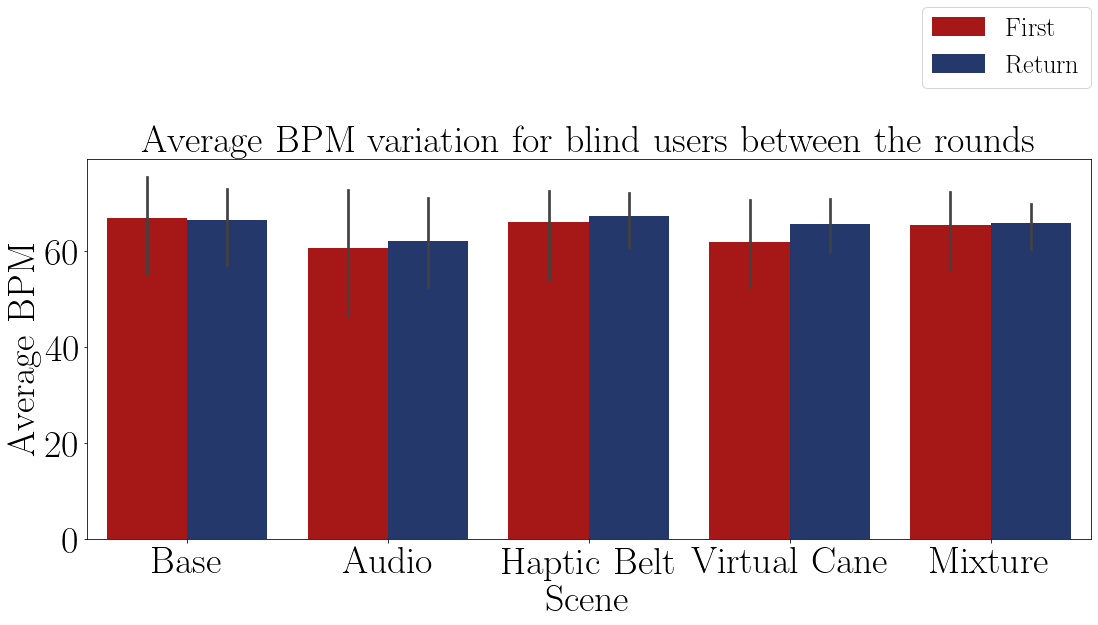
\includegraphics[width = 0.8\linewidth]{Resultados/ECG/Figuras/png/barplot_ecg_bpm_5_scene_blind.png}
    \caption{Barplot of the average BPM of the blind participants on each method.}
    \label{fig:barplot_ecg_bpm_5_scene_blind}
\end{figure}

The Table \ref{tab:bpm_average_group_blind} show the average heartbeat frequency variation between the rounds of each group. As it was shown in the Figure \ref{fig:barplot_ecg_bpm_5_scene_blind}, only the "Base" method has a negative average variaton between the rounds. It is also posible to see that the Virtual Cane variation was the highest, hence it was also the highest mental workload.
 

\begin{table}[!htb]
\centering
\caption{ECG average BPM  for each method of the blind participants.}
\label{tab:bpm_average_group_blind}
\begin{tabular}{lrrrrr}
\toprule
{} &   Base & Audio & Haptic Belt & Virtual Cane & Mixture \\
Visual Condition &        &       &             &              &         \\
\midrule
Blind            &  -0.58 &  1.40 &        1.09 &         3.79 &    0.57 \\
\bottomrule
\end{tabular}
\end{table}



The Figure \ref{fig:boxplot_ecg_bpm_blind_scene} show a comparison between the methods. There is no big difference between them, but it is posible to 
separate them in two groups based on their similarity. One with “Base”, “Haptic Belt” and “Mixture” methods and the other with “Audio” and “Virtual Cane”. The Figure \ref{fig:boxplot_ecg_bpm_blind_rounds} presents the average heartreate frequency grouped by round.

\begin{figure}[!htb]
    \centering
    \begin{minipage}{0.45\textwidth}
        \centering
        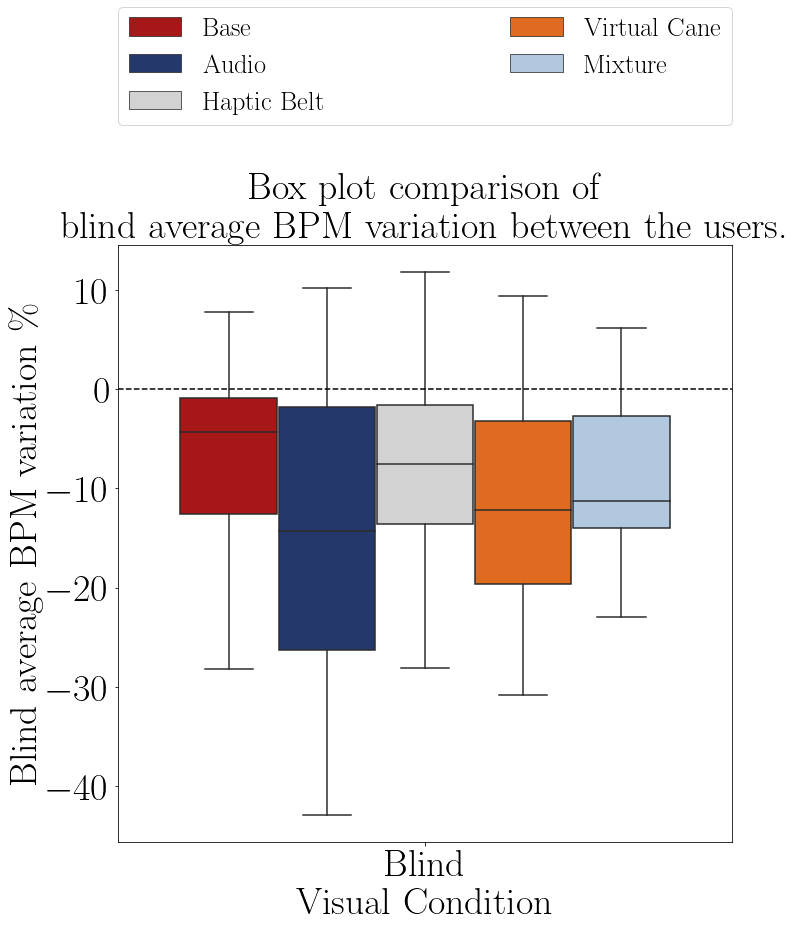
\includegraphics[width = 0.8\linewidth]{Resultados/ECG/Figuras/png/boxplot_ecg_bpm_blind_scene.png}
        \caption{Boxplot of the BPM of the blind participants grouped by method.}
        \label{fig:boxplot_ecg_bpm_blind_scene}
    \end{minipage}
    \begin{minipage}{0.45\textwidth}
        \centering
        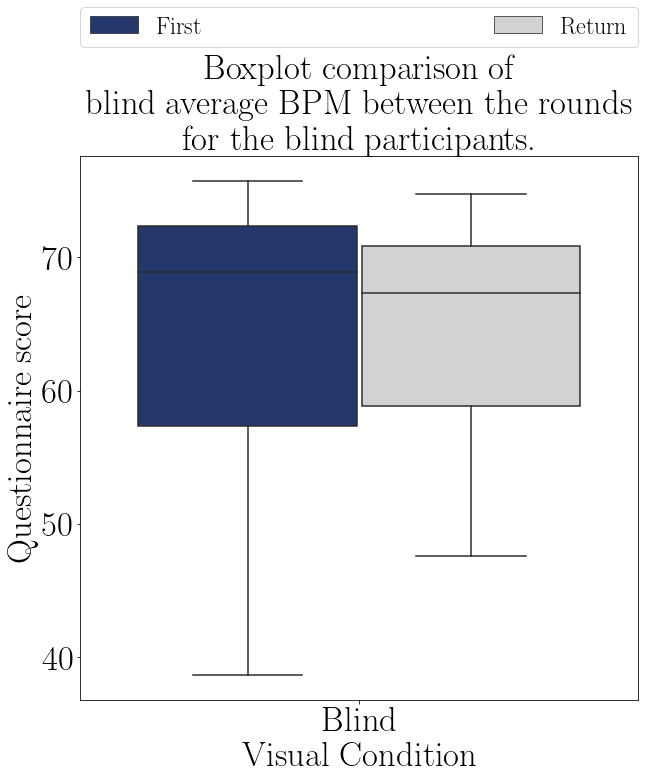
\includegraphics[width = 0.8\linewidth]{Resultados/ECG/Figuras/png/boxplot_ecg_bpm_blind_rounds.png}
        \caption{Boxplot of the BPM of the blind participants grouped by round.}
        \label{fig:boxplot_ecg_bpm_blind_rounds}
    \end{minipage}
\end{figure}

The Figures \ref{fig:qqplot_bpm_two_way} and \ref{fig:residplot_bpm_two_way} shows the distribution and variance of the Table \ref{tab:bpm_table_blind}. These Figures shows that the data are normally distributed but the participants had different  that the methods have a similar variance.
The Table \ref{tab:blocanova_bpm_two_way} shows the ANOVA test p-value of the heart rate frequency of the “blind” sample. The p-value indicates that there is no effect of the methods, rounds and neither their interaction in the heartrate frequency.


\begin{table}[!htb]
\centering
\caption{Anova p-value for the BPM on each method for blinded users.}
\label{tab:blocanova_bpm_two_way}
\begin{tabular}{lrrrrr}
\toprule
               Source &  Squared sum &  DOF & Squared average &      F & \begin{tabular}[c]{@{}l@{}}P-Value \\ $(F_{0} > F)$\end{tabular} \\
\midrule
Participants (Blocks) &     2807.274 &    3 &         935.758 & 49.361 &                                                                  \\
         \    Methods &      164.045 &    4 &          41.011 &  2.163 &                                                            0.100 \\
          \    Rounds &       15.693 &    1 &          15.693 &  0.828 &                                                            0.371 \\
     \    Interaction &       20.606 &    4 &           5.152 &  0.272 &                                                            0.894 \\
   Experimental Error &      511.853 &   27 &          18.958 &        &                                                                  \\
                Total &     3519.471 &   39 &                 &        &                                                                  \\
\bottomrule
\end{tabular}
\end{table}



\begin{figure}[!htb]
    \centering
    \begin{minipage}{0.45\textwidth}
        \centering
        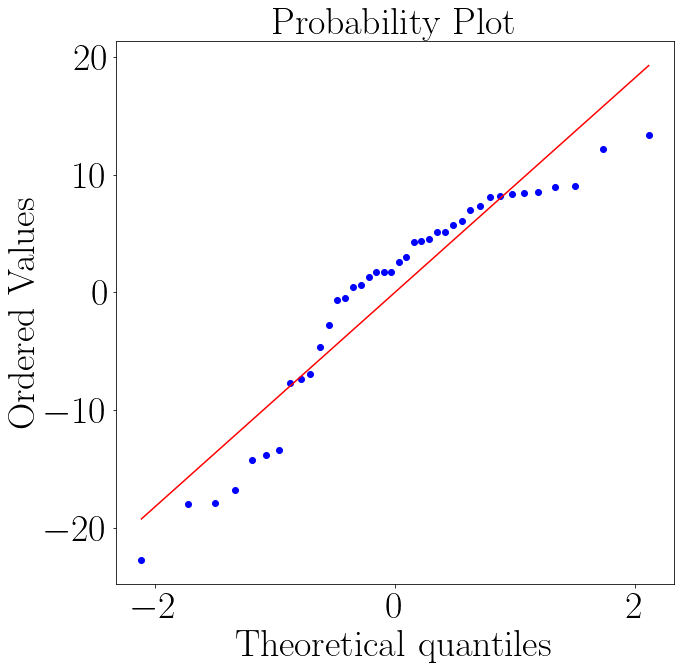
\includegraphics[width = 0.8\linewidth]{Resultados/ECG/Figuras/png/qqplot_bpm_two_way.png}
        \caption{QQ plot of the BPM of the blind participants on each method.}
        \label{fig:qqplot_bpm_two_way}
    \end{minipage}
    \begin{minipage}{0.45\textwidth}
        \centering
        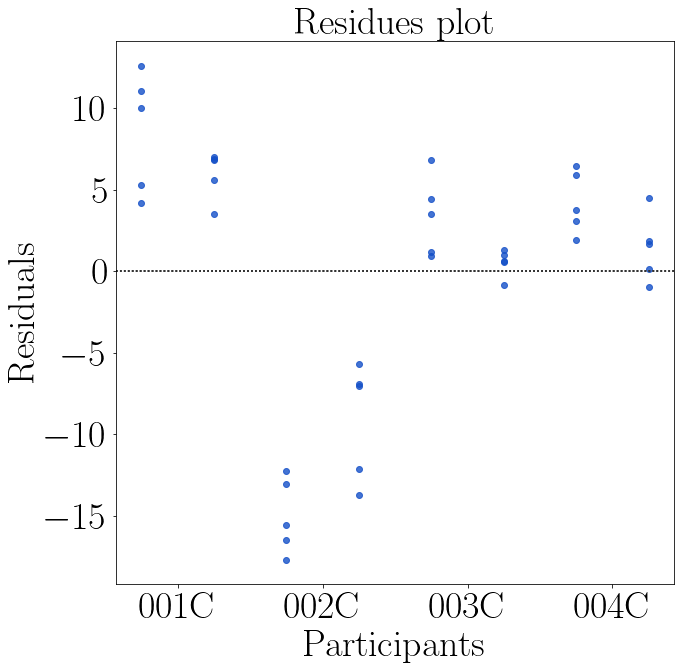
\includegraphics[width = 0.8\linewidth]{Resultados/ECG/Figuras/png/residplot_bpm_two_way.png}
        \caption{Residual plot of the BPM score the blind participants on each method.}
        \label{fig:residplot_bpm_two_way}
    \end{minipage}
\end{figure}


%
\begin{table}[!htb]
\centering
\caption{Cross validation p-value for the average BPM on each method for blinded users.}
\label{tab:lsd_bpm_two_way}
\begin{tabular}{rclr}
\toprule
      \multicolumn{3}{c}{Method} &                                           Analysis \\
\midrule
              Base & $X$ & Audio &               $H_1 : \mu_{Base} \ne \mu_{Audio}**$ \\
        Base & $X$ & Haptic Belt &             $H_0 : \mu_{Base} = \mu_{Haptic Belt}$ \\
       Base & $X$ & Virtual Cane &        $H_1 : \mu_{Base} \ne \mu_{Virtual Cane}**$ \\
            Base & $X$ & Mixture &             $H_1 : \mu_{Base} \ne \mu_{Mixture}**$ \\
       Audio & $X$ & Haptic Belt &        $H_1 : \mu_{Audio} \ne \mu_{Haptic Belt}**$ \\
      Audio & $X$ & Virtual Cane &       $H_1 : \mu_{Audio} \ne \mu_{Virtual Cane}**$ \\
           Audio & $X$ & Mixture &            $H_1 : \mu_{Audio} \ne \mu_{Mixture}**$ \\
Haptic Belt & $X$ & Virtual Cane & $H_1 : \mu_{Haptic Belt} \ne \mu_{Virtual Cane}**$ \\
     Haptic Belt & $X$ & Mixture &      $H_1 : \mu_{Haptic Belt} \ne \mu_{Mixture}**$ \\
    Virtual Cane & $X$ & Mixture &     $H_1 : \mu_{Virtual Cane} \ne \mu_{Mixture}**$ \\
\bottomrule
\end{tabular}
\end{table}



%The Table \ref{tab:lsd_bpm_two_way} presents the conclusion of a pairwise Fisher LSD test of the blind heart rate frequency variation between all the guidance methods. The results show that the only the "Base" and "Haptic belt" have simila reaction.

According to the ANOVA test at Table \ref{tab:blocanova_bpm_two_way}, there is no effect from the method, the round or the interaction between them in the heartrate frequency. It is posible to notice some small difference in the Figure \ref{fig:boxplot_ecg_bpm_blind_scene} but maybe because of the small sample size, it was no sensitive enough to be proved by the ANOVA test.

\FloatBarrier

%%%%%%%%%%%%%%%%%%%%%%%%%%%%%%%%%%%%%%%%%%%%%%%%%%%%%%%%%%%%%%%%%%%%%%%%%%%%
%%%%%%%%%%%%%%%%%%%%%%%%%%%%%%%%%%%%%%%%%%%%%%%%%%%%%%%%%%%%%%%%%%%%%%%%%%%%
%%%%%%%%%%%%%%%%%%%%%%%%%%%%%%%%%%%%%%%%%%%%%%%%%%%%%%%%%%%%%%%%%%%%%%%%%%%%
%%%%%%%%%%%%%%%%%%%%%%%%%%%%%%%%%%%%%%%%%%%%%%%%%%%%%%%%%%%%%%%%%%%%%%%%%%%%
%
%
\paragraph{Analysis of the heartbeat variance (SDNN)}\mbox{}\\
%
The Table \ref{tab:sdnn_table_blind} presents the standard deviation of the interbeat interval by each participant on each scenes. As it was with the Table \ref{tab:bpm_table_blind}, it is not posible to draw a pattern inside this Table. Different participant had increase, or decrease, with different methods.


\begin{table}[!htb]
\centering
\caption{Average SDNN of the blind participants during the each round and method [ms].}
\label{tab:sdnn_table_blind}
\begin{tabular}{llrrrrr}
\toprule
     &        &    Base &   Audio &  \begin{tabular}[c]{@{}l@{}}Haptic\\ Belt\end{tabular} &  \begin{tabular}[c]{@{}l@{}}Virtual\\ Cane\end{tabular} &  Mixture \\
Participant & Round &         &         &                                                        &                                                         &          \\
\midrule
001C & First &  81.292 & 107.061 &                                                124.737 &                                                 163.968 &  129.054 \\
     & Return & 120.719 & 130.885 &                                                131.590 &                                                 157.589 &  124.786 \\
002C & First &  73.761 &  98.863 &                                                 81.140 &                                                  33.977 &   79.289 \\
     & Return & 108.940 &  49.627 &                                                 42.815 &                                                 114.057 &  107.545 \\
003C & First &  36.870 &  38.325 &                                                 35.101 &                                                  42.392 &   43.692 \\
     & Return &  52.750 &  41.196 &                                                 44.256 &                                                  42.602 &   46.145 \\
004C & First &  70.728 &  86.827 &                                                 62.560 &                                                  85.900 &   70.472 \\
     & Return &  71.950 &  74.895 &                                                 70.017 &                                                  66.089 &  104.040 \\
\bottomrule
\end{tabular}
\end{table}



Inside the barplot Figure \ref{fig:barplot_ecg_sdnn_5_scene_blind} shows the average SDNN in each method. It is posible to notice that some method had an increase and some a decrease in the SDNN. The ones that indicate an increase would mean that the participant felt a lesser mental workload in the "Return" round, whilst the deacrese means the opposite.

\begin{figure}[!htb]
    \centering
    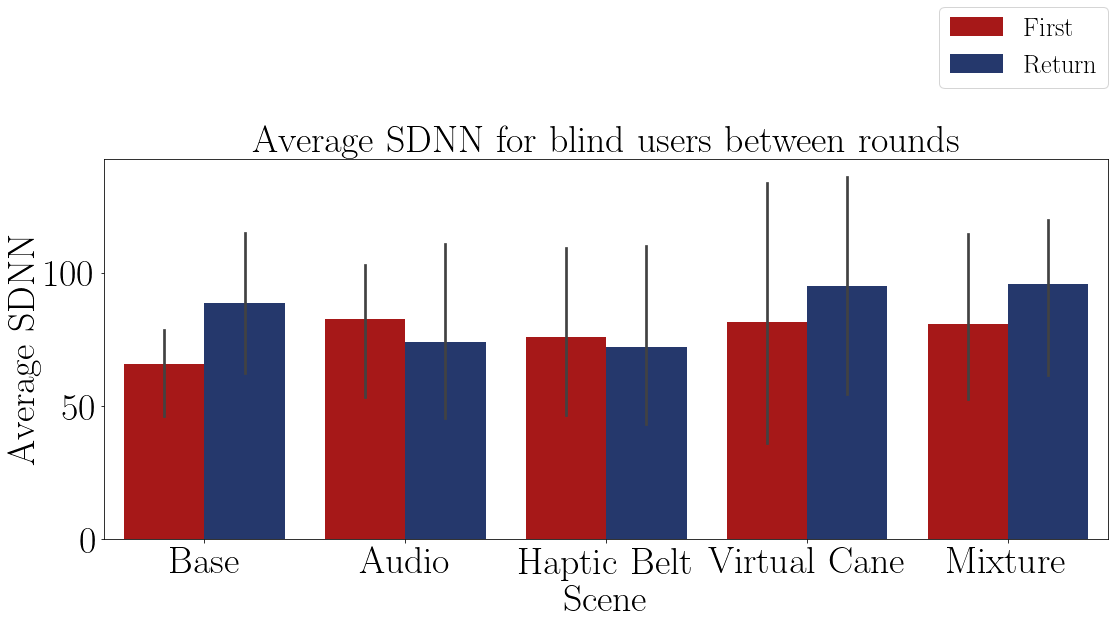
\includegraphics[width = 0.8\linewidth]{Resultados/ECG/Figuras/png/barplot_ecg_sdnn_5_scene_blind.png}
    \caption{Barplot of the average SDNN of the blind participants on each method.}
    \label{fig:barplot_ecg_sdnn_5_scene_blind}
\end{figure}

The Table \ref{tab:sdnn_average_group_blind} presents the average SDNN variation between the rounds. It shows that only the "Audio" and the "Haptic Belt" methods shown a increase in the mental workload.


\begin{table}[!htb]
\centering
\caption{ECG average SDNN for each method of the blind participants.}
\label{tab:sdnn_average_group_blind}
\begin{tabular}{lrrrrr}
\toprule
{} &   Base &  Audio & Haptic Belt & Virtual Cane & Mixture \\
Visual Condition &        &        &             &              &         \\
\midrule
Blind            &  77.13 &  78.46 &       74.03 &        88.32 &   88.13 \\
\bottomrule
\end{tabular}
\end{table}



The Figures \ref{fig:boxplot_ecg_sdnn_blind_scene} presents the distribution of each method SDNN. It noticeable that the "Base" method has a different SDNN than the rest. The "Virtual Cane" also has a different distribution from the rest. The Figure \ref{fig:boxplot_ecg_sdnn_blind_rounds} presents the SDNN grouped by the rounds. It shows a slight difference between the rounds.


\begin{figure}[!htb]
    \centering
    \begin{minipage}{0.45\textwidth}
        \centering
        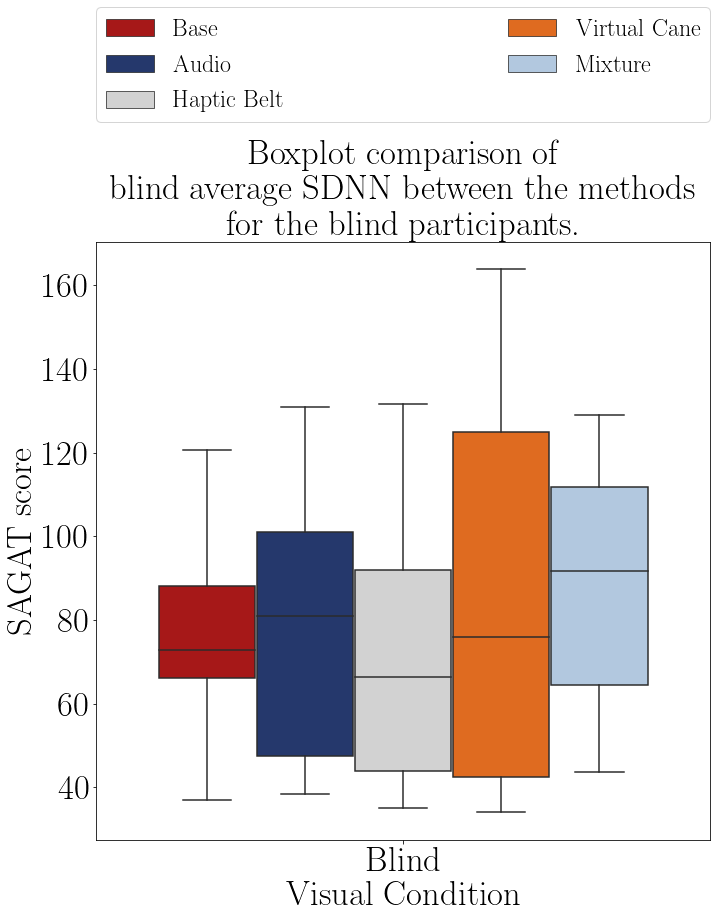
\includegraphics[width = 0.8\linewidth]{Resultados/ECG/Figuras/png/boxplot_ecg_sdnn_blind_scene.png}
        \caption{Boxplot of the SDNN of the blind participants grouped by method.}
        \label{fig:boxplot_ecg_sdnn_blind_scene}
    \end{minipage}
    \begin{minipage}{0.45\textwidth}
        \centering
        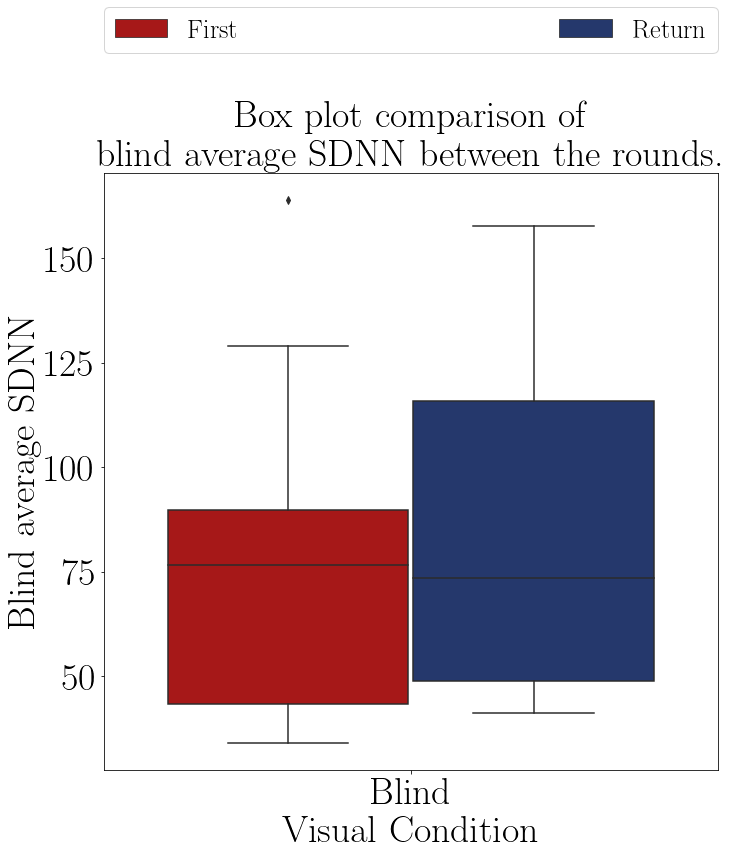
\includegraphics[width = 0.8\linewidth]{Resultados/ECG/Figuras/png/boxplot_ecg_sdnn_blind_rounds.png}
        \caption{Boxplot of the SDNN of the blind participants grouped by round.}
        \label{fig:boxplot_ecg_sdnn_blind_rounds}
    \end{minipage}
\end{figure}

The Figures \ref{fig:qqplot_sdnn_two_way} and \ref{fig:residplot_sdnn_two_way} shows the distribution and variance of the Table \ref{tab:sdnn_table_blind}. These Figures shows that the data are normally distributed but the participants had different  that the methods have a similar variance.
The Table \ref{tab:blocdanova_sdnn_two_way} shows the ANOVA test p-value of the heartbeat interval variance of the “blind” sample. The p-value indicates that there is no effect of any factor.


\begin{table}[!htb]
\centering
\caption{Anova p-value for the average SDNN on each method for blinded users.}
\label{tab:blocdanova_sdnn_two_way}
\begin{tabular}{lrrrrr}
\toprule
               Source &  Squared sum &  DOF & Squared average &      F & \begin{tabular}[c]{@{}l@{}}P-Value \\ $(F_{0} > F)$\end{tabular} \\
\midrule
Participants (Blocks) &    36520.955 &    3 &       12173.652 & 30.932 &                                                                  \\
         \    Methods &     1394.166 &    4 &         348.542 &  0.886 &                                                            0.486 \\
          \    Rounds &      612.182 &    1 &         612.182 &  1.555 &                                                            0.223 \\
     \    Interaction &     1431.284 &    4 &         357.821 &  0.909 &                                                            0.473 \\
   Experimental Error &    10626.244 &   27 &         393.565 &        &                                                                  \\
                Total &    50584.831 &   39 &                 &        &                                                                  \\
\bottomrule
\end{tabular}
\end{table}



\begin{figure}[!htb]
    \centering
    \begin{minipage}{0.45\textwidth}
        \centering
        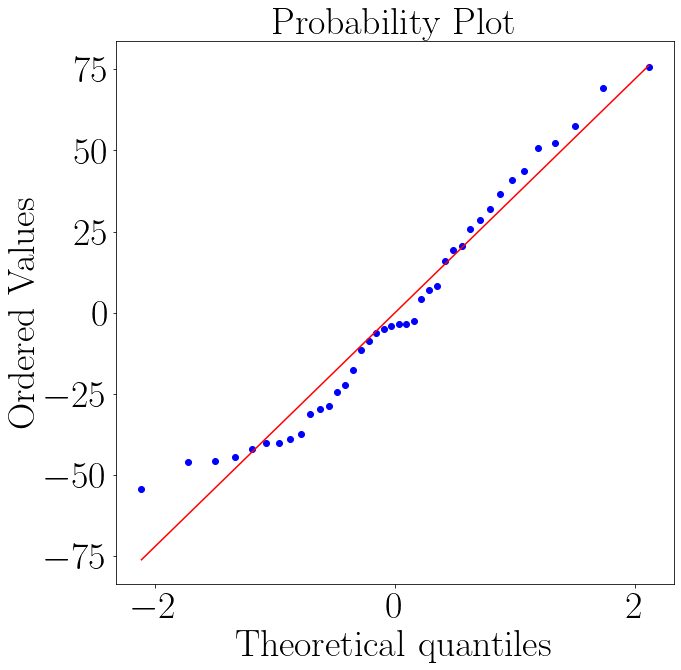
\includegraphics[width = 0.8\linewidth]{Resultados/ECG/Figuras/png/qqplot_sdnn_two_way.png}
        \caption{QQ plot of the SDNN of the blind participants on each method.}
        \label{fig:qqplot_sdnn_two_way}
    \end{minipage}
    \begin{minipage}{0.45\textwidth}
        \centering
        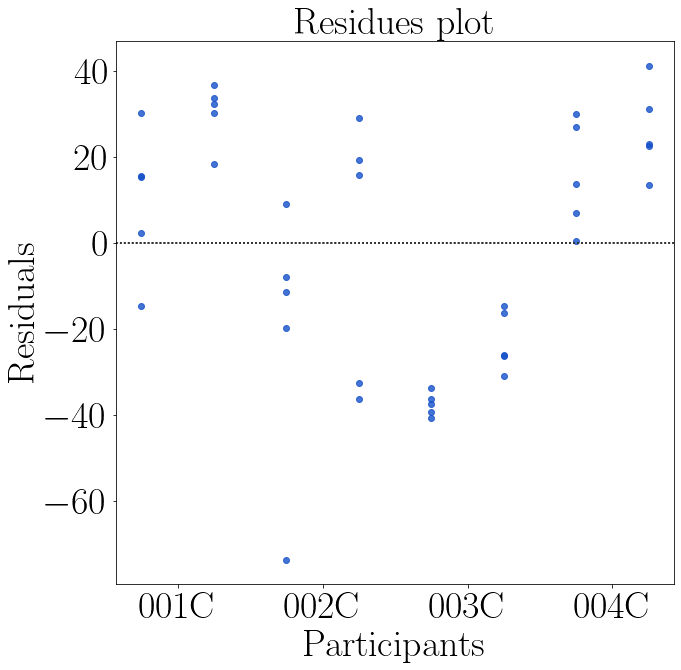
\includegraphics[width = 0.8\linewidth]{Resultados/ECG/Figuras/png/residplot_sdnn_two_way.png}
        \caption{Residual plot of the SDNN of the blind participants on each method.}
        \label{fig:residplot_sdnn_two_way}
    \end{minipage}
\end{figure}

%
\begin{table}[!htb]
\centering
\caption{Cross validation p-value for the average SDNN on each method for blinded users.}
\label{tab:lsd_sdnn_two_way}
\begin{tabular}{rclr}
\toprule
      \multicolumn{3}{c}{Method} &                                           Analysis \\
\midrule
              Base & $X$ & Audio &                   $H_0 : \mu_{Base} = \mu_{Audio}$ \\
        Base & $X$ & Haptic Belt &             $H_0 : \mu_{Base} = \mu_{Haptic Belt}$ \\
       Base & $X$ & Virtual Cane &        $H_1 : \mu_{Base} \ne \mu_{Virtual Cane}**$ \\
            Base & $X$ & Mixture &             $H_1 : \mu_{Base} \ne \mu_{Mixture}**$ \\
       Audio & $X$ & Haptic Belt &        $H_1 : \mu_{Audio} \ne \mu_{Haptic Belt}**$ \\
      Audio & $X$ & Virtual Cane &       $H_1 : \mu_{Audio} \ne \mu_{Virtual Cane}**$ \\
           Audio & $X$ & Mixture &            $H_1 : \mu_{Audio} \ne \mu_{Mixture}**$ \\
Haptic Belt & $X$ & Virtual Cane & $H_1 : \mu_{Haptic Belt} \ne \mu_{Virtual Cane}**$ \\
     Haptic Belt & $X$ & Mixture &      $H_1 : \mu_{Haptic Belt} \ne \mu_{Mixture}**$ \\
    Virtual Cane & $X$ & Mixture &         $H_0 : \mu_{Virtual Cane} = \mu_{Mixture}$ \\
\bottomrule
\end{tabular}
\end{table}



The Table \ref{tab:blocdanova_sdnn_two_way} does not prove that any method or round has some influence in the heartbeat interval variance, thus in the Mental Workload. Although, in the Figure \ref{fig:boxplot_ecg_sdnn_blind_scene} it is posible to notice that the "Base" method has a different distribution. As it has already commented before, maybe the result of the anova test is a conseguence of a small sample size.

\FloatBarrier